%! TEX program = lualatex

\documentclass[nobackground,dvipsnames,table]{beamer}
\usepackage{sio}

\mode<presentation>
{\usetheme{Hannover}
    \usecolortheme{sio}
    \setbeamercovered{transparent}
    \useinnertheme[shadow=false]{rounded}
    \usebackgroundtemplate{}
    \setbeamercolor*{frametitle}{parent=palette primary}
    \setbeamerfont{block title}{size={}}
    \setbeamertemplate{navigation symbols}{}
}

\title{An Introduction to Trust and Safety}
\subtitle{CS 152 - Lecture 1}

\author[A. Stamos]{Alex Stamos}
\institute[SIO]{\large Stanford Internet Observatory}
\date[2022]{\today}
\subject{CS 152 - Trust and Safety Engineering}
\titlegraphic{
\includegraphics[width=5cm]{img/internet-observatory}}

% Change the level of bulleting on the ToC page
\setcounter{tocdepth}{2}

\graphicspath{{img/lesson01}}

\begin{document}

\coverpage

\begin{frame}
    \titlepage
\end{frame}

\section{What is Trust and Safety?}

\begin{frame}{What will we learn today?}
    Today, we will...
    \begin{itemize}
        \item Discuss the practical aspects of this class
        \item Explore how Trust and Safety differs from other areas of tech risk
        \item Start to understand the Trust and Safety lifecycle
    \end{itemize}
\end{frame}

\begin{frame}{} %TODO3: Teaching Team slide - not sure how to implement
    \thispagestyle{empty}
    \huge
    Teaching Team
\end{frame}

\begin{frame}{Our Agenda}
    %TODO2: update schedule then make it look nicer
    \footnotesize
    \begin{columns}[t]
        \column{0.5\textwidth}
                    Mon, Jan 3 - Introduction to Trust \& Safety \\
                    Wed, Jan 5 - How Tech Companies Work. Designing for Trust, Safety \& Privacy \\
                    Mon, Jan 10 - Authentication \& Identity \\
                    Wed, Jan 12 - Guest Lecture: Fraud \\
                    Mon, Jan 17 - HOLIDAY \\
                    Wed, Jan 19 - Spam, Fraud \& Cybercrime \\
                    Mon, Jan 24 - Surveillance, Government Oppression \& Domestic Abuse \\
                    Wed, Jan 27 - Harassment, Bullying \& Threatening Behavior \\
                    Mon, Jan 31 - Hate Speech \& Extremism  \\
                    Wed, Feb 2 - Incitement \& Terrorism \\
                    Mon, Feb 7 - Suicide \& Self-Harm \\
                    Wed, Feb 9 - Child \& Adult Sexual Exploitation I - CSAM, NCII \& Responses \\
            \column{0.5\textwidth}
                    Mon, Feb 14 - Child \& Adult Sexual Exploitation II - Grooming, Sextortion \& Trafficking \\
                    Wed, Feb 16 - Working with Law Enforcement \& CSE Case Studies \\
                    Mon, Feb 21 - HOLIDAY \\
                    Wed, Feb 23 - Misinformation \& Disinformation \\
                    Mon, Feb 28 - Case Study: The 2016 \& 2020 US Elections \\
                    Wed, Mar 2 - Guest Lecture: TBD \\
                    Mon, Mar 7 - Content Moderation \& Resiliency \\ 
                    Wed, Mar 9 - Sharing Economy, Emerging Issues \& Career Advice \\
                    Mar 14-18 - Final Presentations, To Be Scheduled \\
        \end{columns}
\end{frame}

\begin{frame}{Who should take this class?}
    Students who:
    \begin{enumerate}
        \item Are interested in the ways technology can be abused to cause harm
        \item Want to build consumer internet products more safely
        \item Who are interested in careers in Trust and Safety, anti-abuse NGOs, law enforcement or internet policy
        \item Who can participate in the group project at a 106B level
    \end{enumerate}

    We now have a partner class, POLISCI 243C: The Politics of Internet Abuse
\end{frame}

\begin{frame}{Project Teams + Sections}
    Project teams
    \begin{itemize}
        \small
        \item Teams of four CS students, one POLISCI
        \item Class intro form will be sent out tomorrow on Ed
        \begin{itemize}
            \item Denote whether you want to be matched into a group OR state your group
        \end{itemize}
        \item Fill those out by \textbf{Friday at noon} - teams will be announced shortly after
    \end{itemize}
    
    Sections will start next week
    \begin{itemize}
        \small
        \item TA facilitated work sessions
        \item Optional, but highly encouraged 
        \item Starting week 2 - times being finalized (check syllabus + Discord)
        \item You don't have to officially sign up, but your whole group should be able to attend together
    \end{itemize}
\end{frame}

\begin{frame}{Grading}
    \textbf{Course Grading}
    \begin{itemize}
        \item Lecture participation and pre-lecture quizzes - 30\%
        \item Project Milestone 1 - 20\%
        \item Project Milestone 2 - 20\%
        \item Project - Final presentation - 30\% \\
    \end{itemize}
    
    \textbf{Final Project}
    \begin{itemize} %TODO2 update deadlines?
        \item \textbf{Milestone 1:} User Studies and Reporting Flow Design (20\%) [Due 2/4]
        \item \textbf{Milestone 2:} Content Moderation App Implementation (20\%) [Due 2/25]
        \item \textbf{Final:}  Incident Response and Final Preso (30\%) [Due 3/11]
    \end{itemize}
\end{frame}

\begin{frame}{Pre-Reading}
    Pre-reads and short reading quizzes before \bfseries every \mdseries class
    \begin{itemize}
        \item Pre-reads will go up a week in advance
        \item Quizzes will go up after previous class
    \end{itemize}
    Readings can be found \underline{\href{https://docs.google.com/document/d/1ljWErgPIRi3ZH4I_iuqqlWF8bERIiDPdakzyjxUccPo/edit}{here}} %TODO2 update link for this year's reading?
    %TODO1 change link color
\end{frame}

\begin{frame}{Attendance Policy}
    \begin{itemize}
        \item Students are welcome to take the class for credit, even if they can't attend the lectures synchronously. I will not boot you out for non-attendance, but I also will not make any grading exceptions.
        \item 30\% of your grade will come from class participation. Half from synchronous attendance quizzes that will only be available at the start of the lecture (and gaming this would be an Honor Code violation) and half from asynchronous quizzes on the pre-reads.
        \item This means that a student who attends zero lectures can get a max of 85\% in the class. That's a B. 
        \item \bfseries I strongly suggest that students who can't make most of the lectures take the class C/NC. \mdseries
        If you take the asynchronous quizzes and your team completes the project, there is really no chance you won't pass (>60\%).
    \end{itemize}
\end{frame}

\section{Learning Goals}

\begin{frame}{} %TODO3: Learning goals slide
    \thispagestyle{empty}
    
    \huge
    Learning Goals
\end{frame}


\begin{frame}{} %TODO2 fix sizing so all of image fits? + caption
    \thispagestyle{empty}
    \centering
    \AddToShipoutPictureBG*{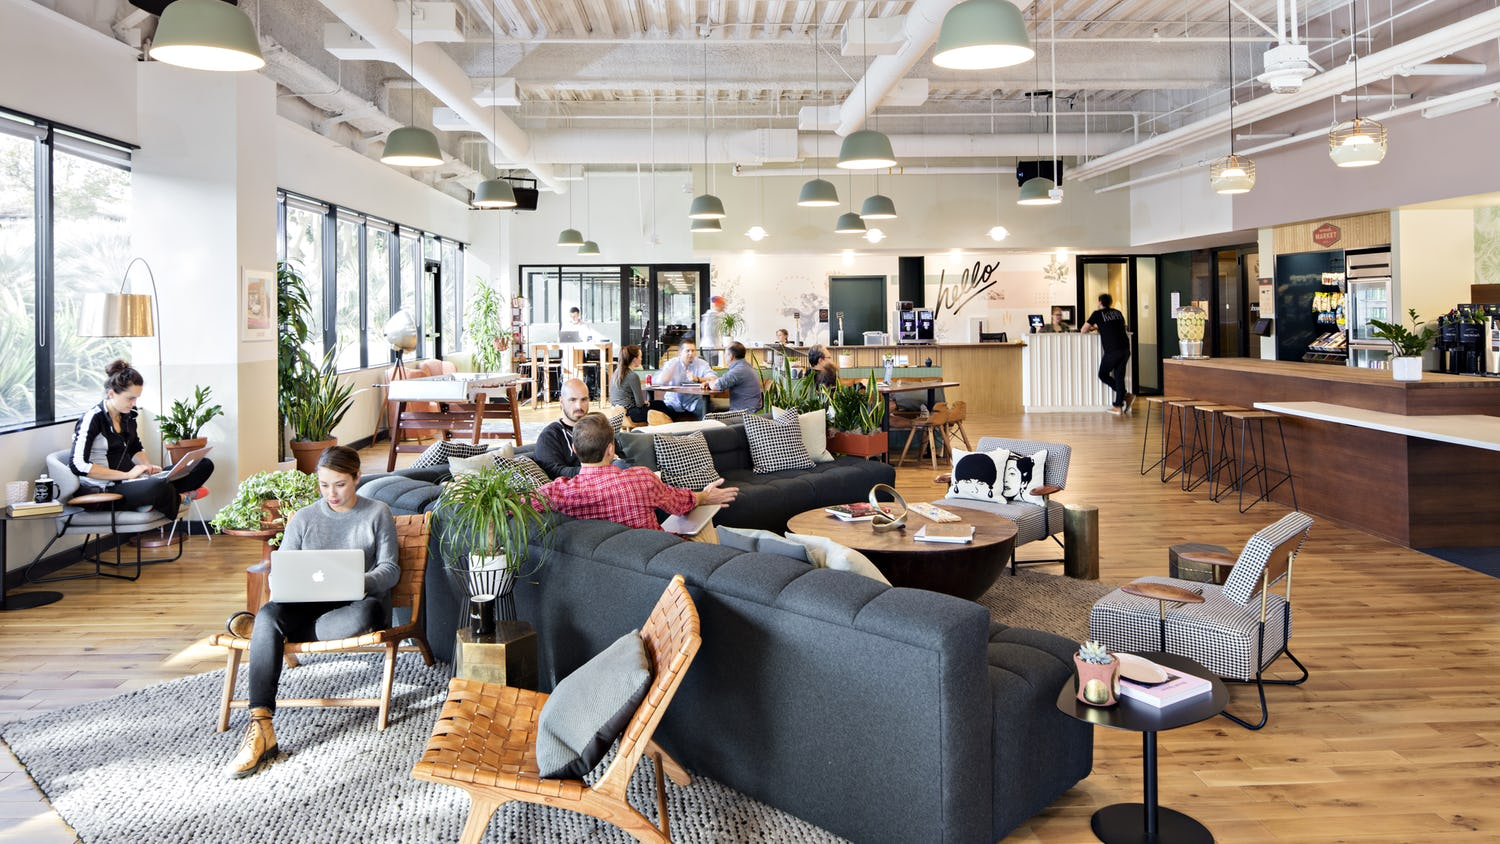
\includegraphics[height=\paperheight]{workspace.png}}
    %Explain to your fellow software engineers and product managers the common ways that internet technologies are used to cause harm.
\end{frame}


\begin{frame}{} %TODO2 how to make free-floating text box for caption
    \thispagestyle{empty}
    \centering
    \AddToShipoutPictureBG*{
\includegraphics[height=\paperheight]{alex-jones-yelling.png}}
    %Recognize the pattern of how long-existing societal challenges (hate speech, disinformation, child abuse) can be changed or amplified by modern communication platforms.
\end{frame}

\begin{frame}{} %TODO2 caption
    \thispagestyle{empty}
    \centering
    \AddToShipoutPictureBG*{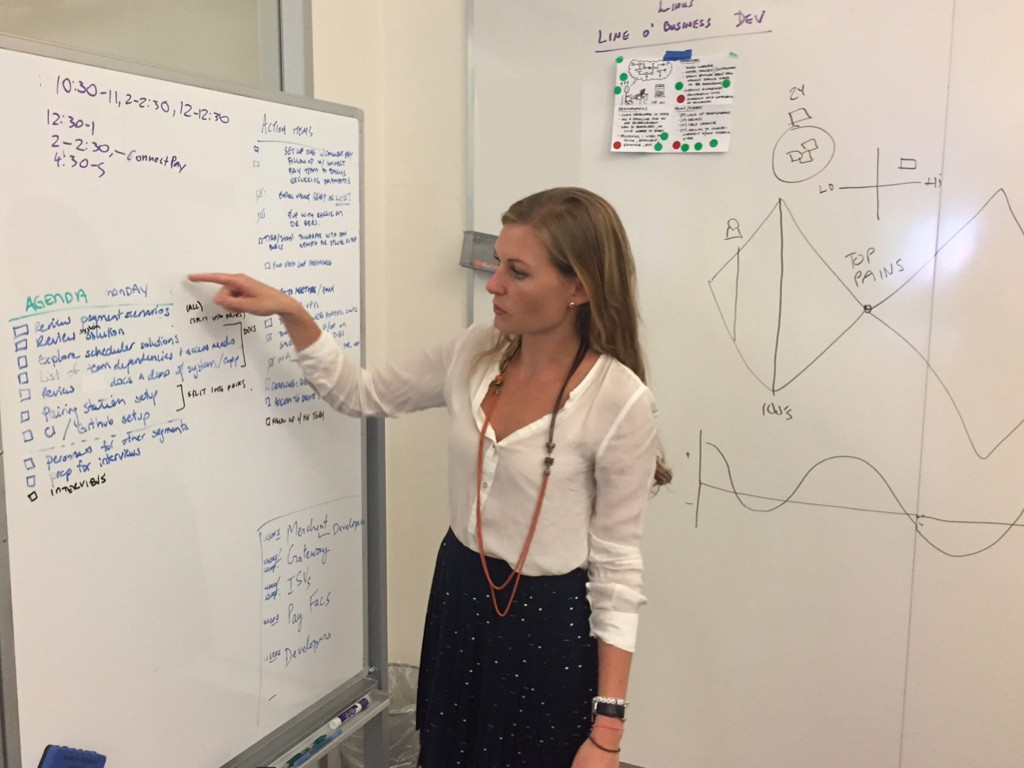
\includegraphics[width=\paperwidth]{whiteboard.png}}
    %Understand how to anticipate safety risks for a proposed product.
\end{frame}

\begin{frame}{} %TODO2 fix sizing/formatting/centering to get rid of blank space OR fill it with black background; caption
    \thispagestyle{empty}
    \centering
    \AddToShipoutPictureBG*{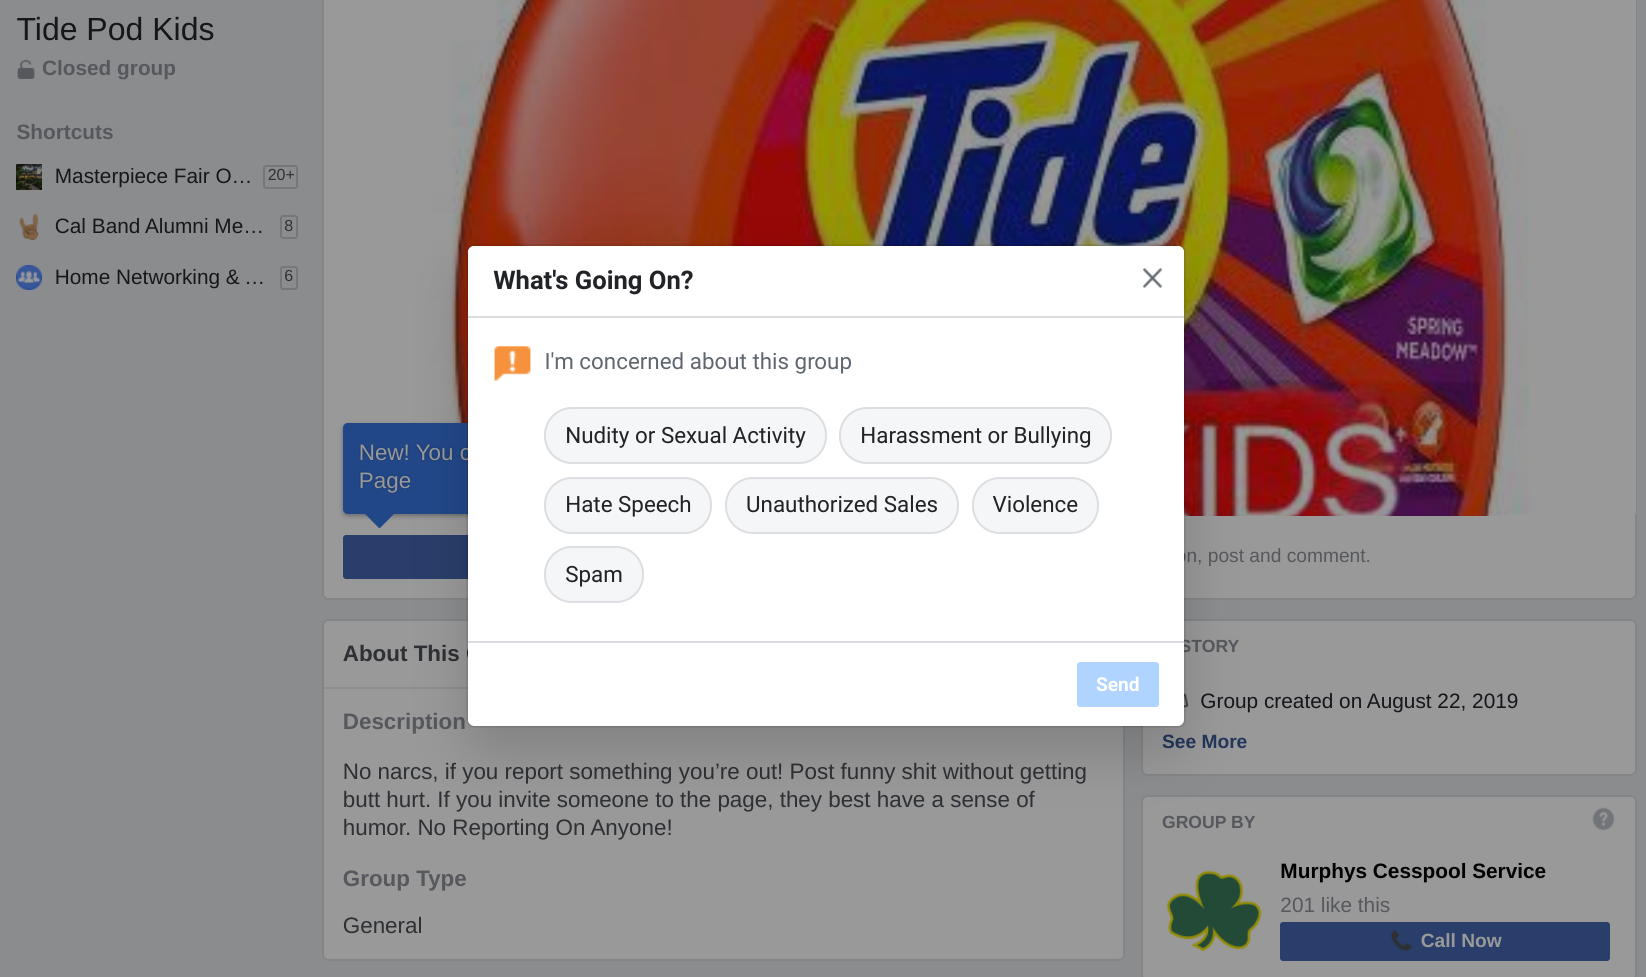
\includegraphics[width=\paperwidth]{tide-pod-facebook-group.png}}
    %Design and implement a functional abuse reporting flow powered by a machine learning classifier.
\end{frame}

\begin{frame}{} %TODO2 caption
    \thispagestyle{empty}
    \centering
    \AddToShipoutPictureBG*{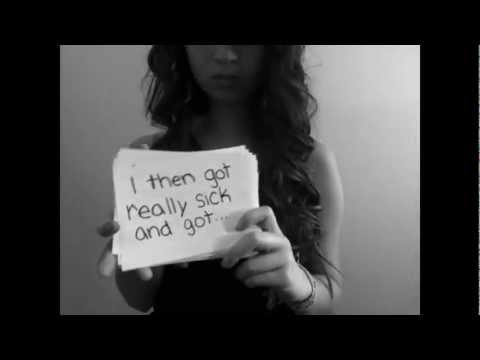
\includegraphics[width=\paperwidth]{got-really-sick.png}} %TODO2 embed video if still available
    %Have empathy for a broad cross-section of the people who use your products and the risks they face.
\end{frame}

\begin{frame}{Dealing with difficult content} %TODO1 change formatting?
    \footnotesize
    The subject matter of this course can be difficult intellectually and emotionally.  We will read about and discuss difficult topics, including (but not limited to) sexual exploitation of adults and minors, harassment, bullying, hate speech, domestic abuse, terrorism, and more. \\ 
    If you anticipate acute distress as a result of encountering a particular topic, talk to me ahead of time to arrange an alternative written assignment in lieu of your in-class participation. If you become so distressed that you need to leave during class, feel free to do so. If you need to leave a class, talk to me afterward and we can arrange an alternate assignment.  I will not “warn” students about particular topics, because sensitivity to different topics varies from person to person, and because topics may arise unexpectedly in class discussion. Please refer to the course agenda to see the list of course topics. \\
    Additionally, as you may know, there is a difference between being triggered (in the sense of post-traumatic stress disorder) and feeling uncomfortable. One of the goals of this class is to help students develop empathy for victims of online abuse. Feeling uncomfortable (and sometimes even angry or offended) is part of intellectual growth. Feeling triggered or psychologically traumatized is not. Please take care of yourselves and each other, and let me know if I can do anything at all to help.
\end{frame}

\begin{frame}{An example of difficult content from a previous project}
    %TODO2 make it larger while still fitting on slide?
    \begin{figure}
        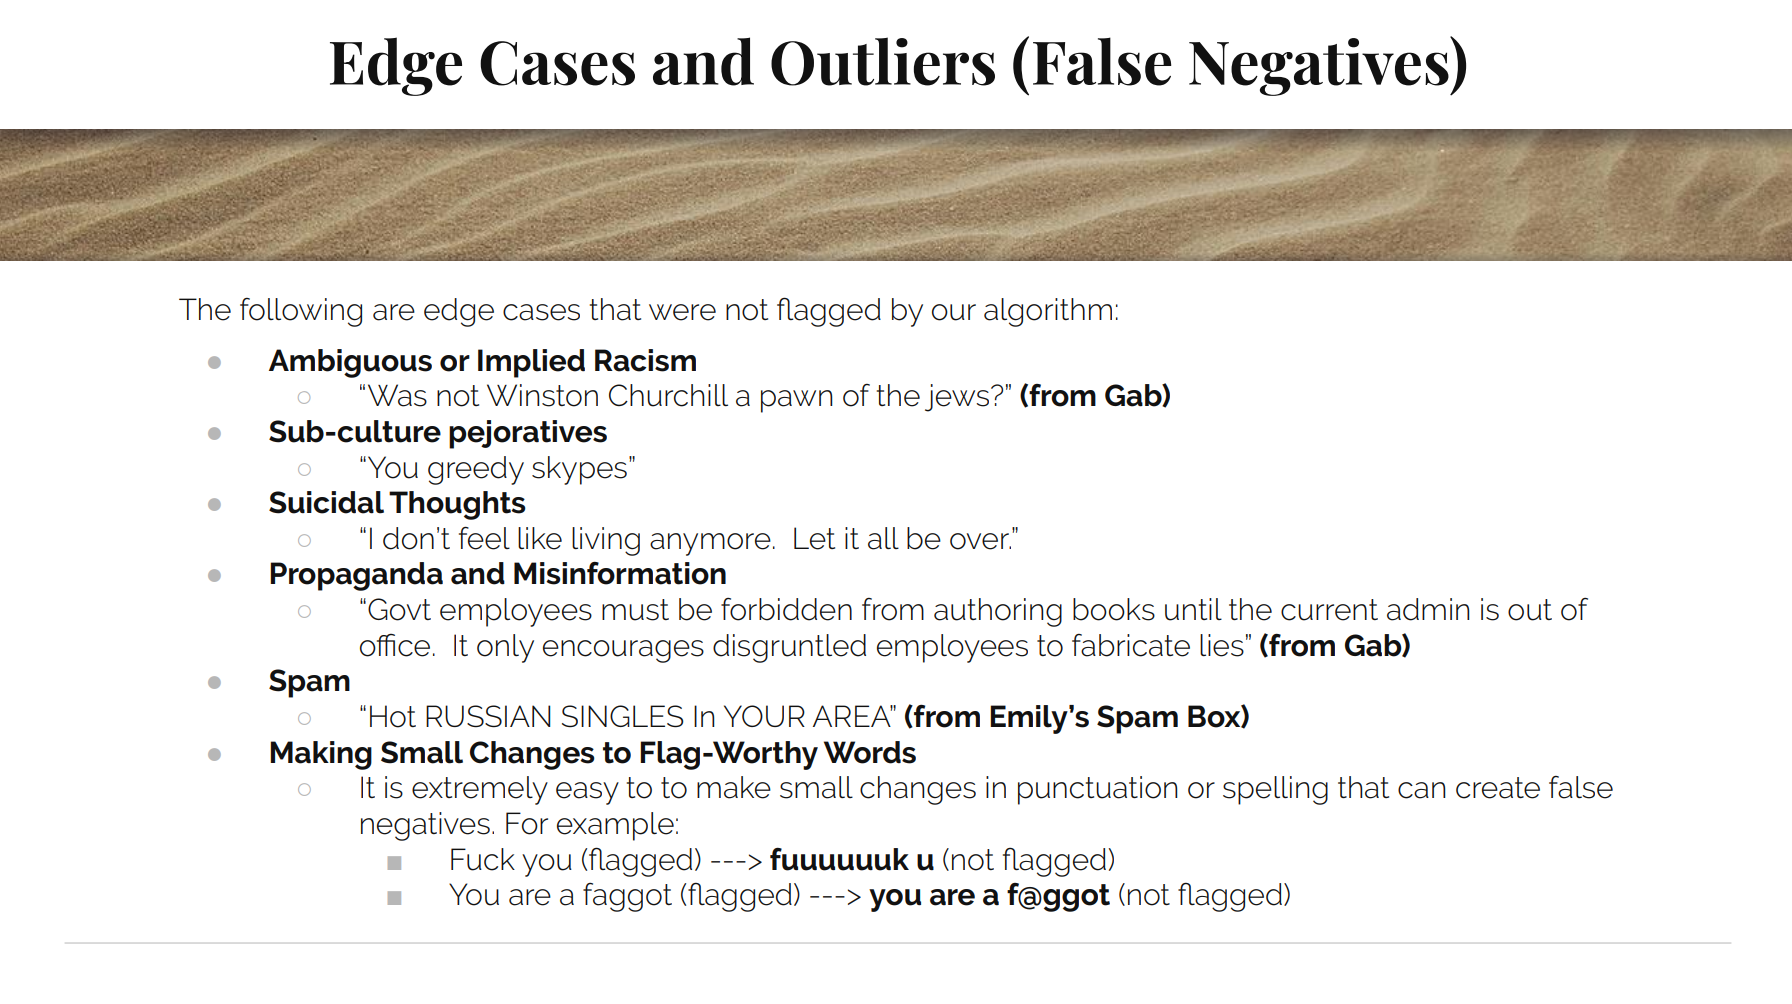
\includegraphics[width=\textwidth]{edge-cases-and-outliers.png}
        \label{edge-cases}
    \end{figure}
\end{frame}


\section{What is Trust and Safety Engineering?}

\begin{frame}{} %TODO3: What is Trust and Safety Engineering? slide - not sure how to implement
    \thispagestyle{empty}
    What is Trust and Safety Engineering?
\end{frame}

\begin{frame}{Unique Aspects of Trust and Safety}
    \begin{columns}
        \column{0.5\textwidth}
            \begin{enumerate}
                \item The study of how people abuse the internet to cause harm.
                \item Often using products the way they are designed to work.
                \item Crosses between specialties. Requires understanding of society and humanity.
                \item Is dynamic and unpredictable. 
            \end{enumerate}
        \column{0.5\textwidth}
            \begin{figure}
                \centering
                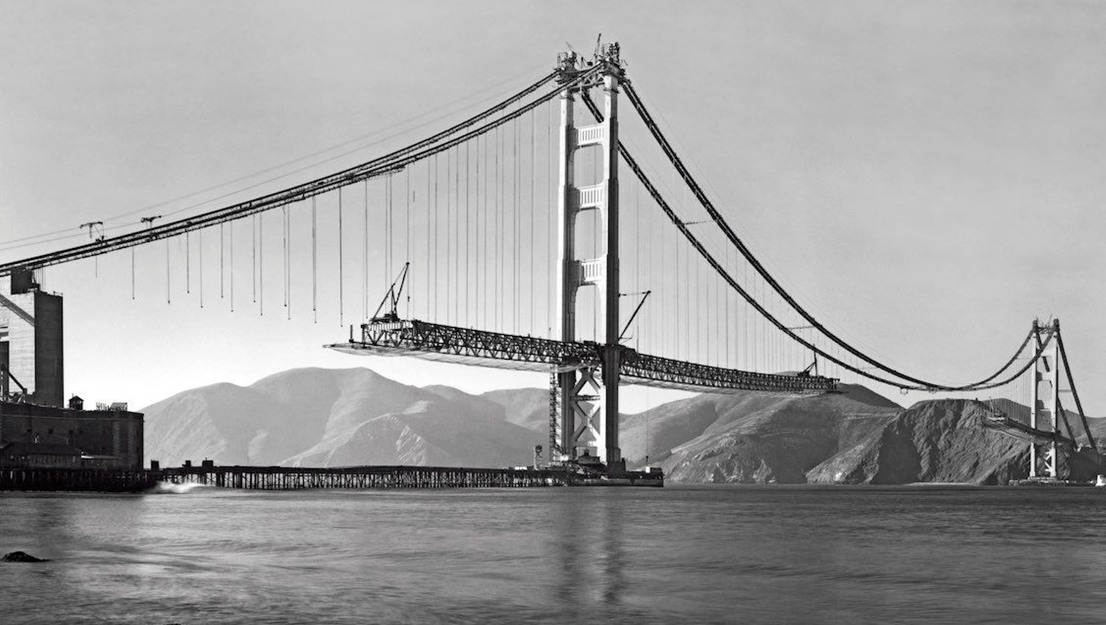
\includegraphics[width=\textwidth]{bridge-construction}
                
\includegraphics[width=\textwidth]{chess}
            \end{figure}
        \end{columns}
\end{frame}

%TODO2: 3 slides with diagrams made in Slides
\begin{frame}{}
    \thispagestyle{empty}
\end{frame}

\begin{frame}{}
    \thispagestyle{empty}
\end{frame}

\begin{frame}{}
    \thispagestyle{empty}
\end{frame}

\begin{frame}{The Biggest Challenges in Trust and Safety}
        \begin{columns}
            \column{0.3\textwidth}
                \begin{figure}
                    \centering
                    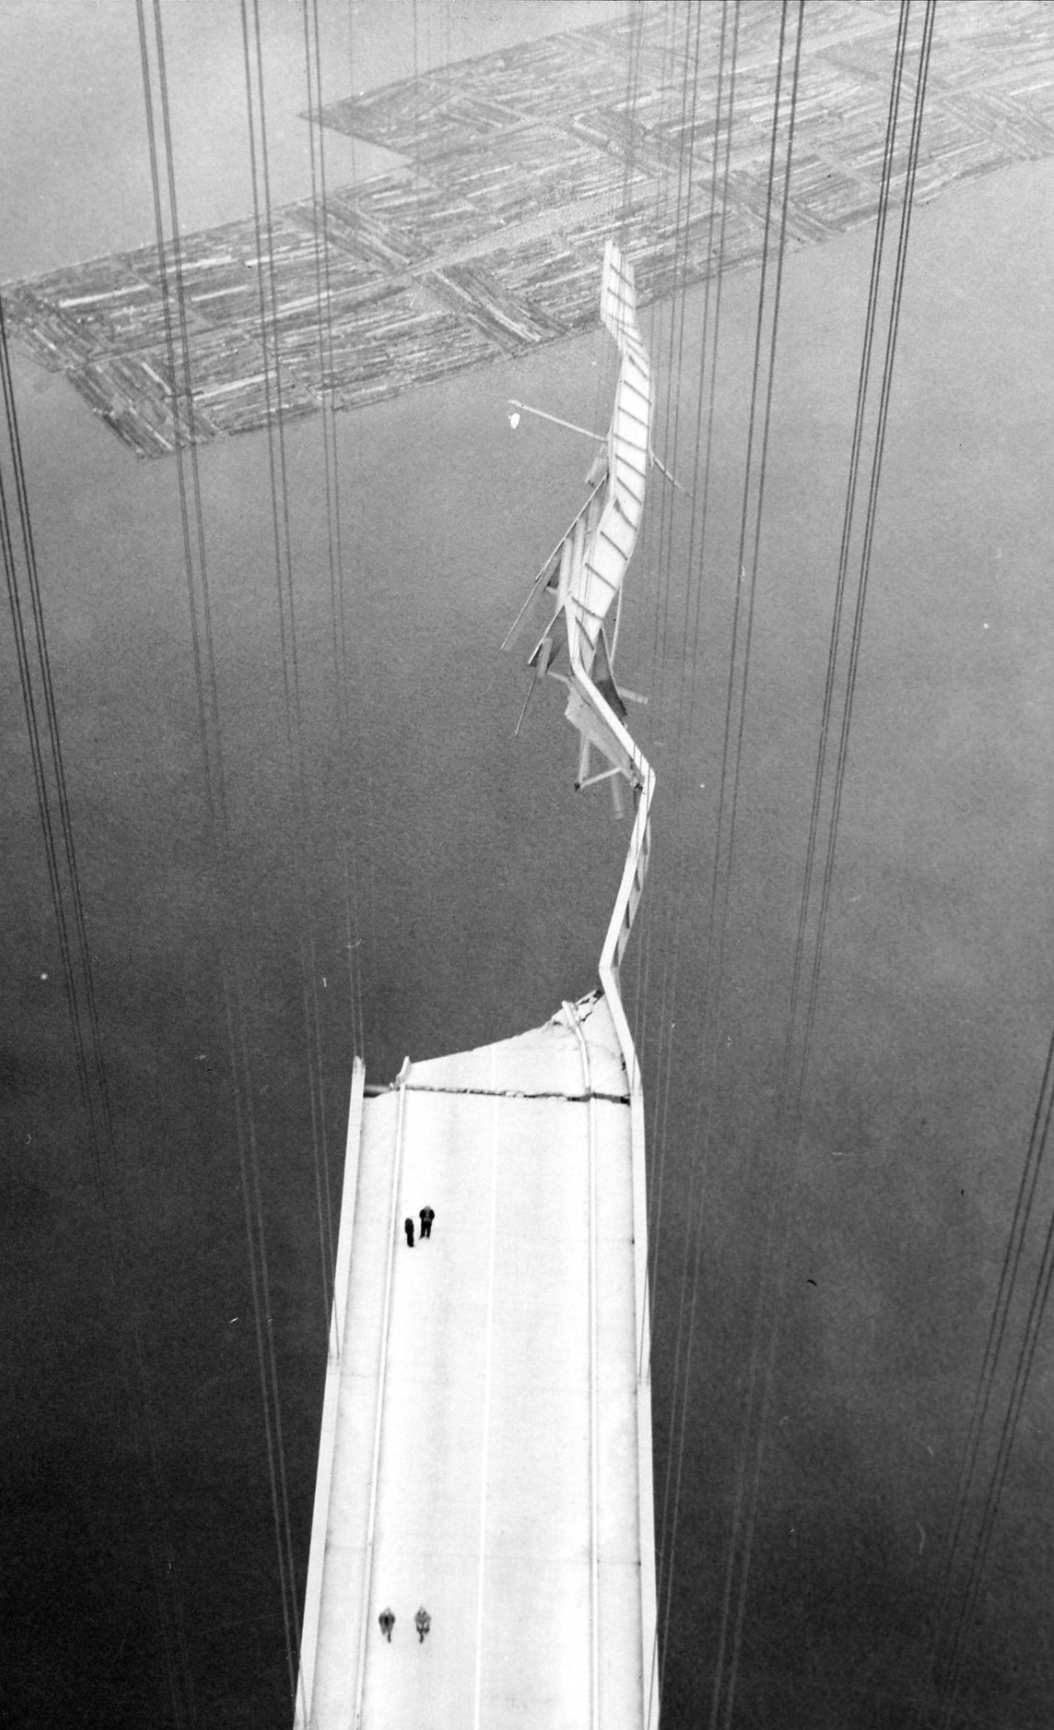
\includegraphics[width=\textwidth]{broken-bridge.png}
                \end{figure}
            \column{0.7\textwidth}
                \begin{enumerate}
                    \item Scale
                    \item Non-diverse studies and solutions
                    \item Measurement and definition challenges
                    \item Privacy vs Safety
                    \item Information sharing and division of responsibility
                    \item Government vs private action
                    \item Fairness in ML solutions
                    \item Freedom of expression
                \end{enumerate}
        \end{columns}
\end{frame}


\section{Who are the Players?}

\begin{frame}{}
        %TODO3: center with respect to slide and not text box change bg color to primary slide color (cardinal red)
        \thispagestyle{empty}
        %\setbeamercolor{background canvas}{bg=cardinalred}
        \huge
        Who are the Players?
\end{frame}

\begin{frame}{Areas of Trust and Safety Work}
    \small
    \begin{columns}[T]
        \column{0.25\textwidth}
            \textbf{Research}\\~\\
            \scriptsize
            Defining abuse types\\~\\
            Building measurements and metrics\\~\\
            Performing field studies\\~\\
            Interviewing users and victims\\~\\
            Provides data and ideas to product
        \column{0.25\textwidth}
            \textbf{Product and Engineering} \\
            \scriptsize
            Red teaming product designs \\~\\
            Designing UX that encourage good behavior \\~\\
            Building detection and moderation mechanisms \\~\\
            Building and training ML
        \column{0.25\textwidth}
            \textbf{Operations} \\~\\
            \scriptsize
            Defining appropriate behavior \\~\\
            Building operational pipelines \\~\\
            Sorting and handling billions of events \\~\\
            Implementing constant improvement through various self-testing
        \column{0.25\textwidth}
            \textbf{Investigations} \\~\\
            \scriptsize
            Investigates worst cases or most effective bad guys \\~\\
            Handles incoming LE requests and external referrals \\~\\
            Applies lessons learned to future operational and product improvements
    \end{columns}
\end{frame}

\begin{frame}{} %TODO3 company/org slide
    \thispagestyle{empty}
\end{frame}

\section{Some Real Cases}

\begin{frame}{} %TODO3: Some Real Questions
    \thispagestyle{empty}
    \huge
    Some Real Cases
\end{frame}

\begin{frame}{Ronan Hughes}
    \begin{columns}
        \column{0.5\textwidth}
            \begin{figure}
                \centering
                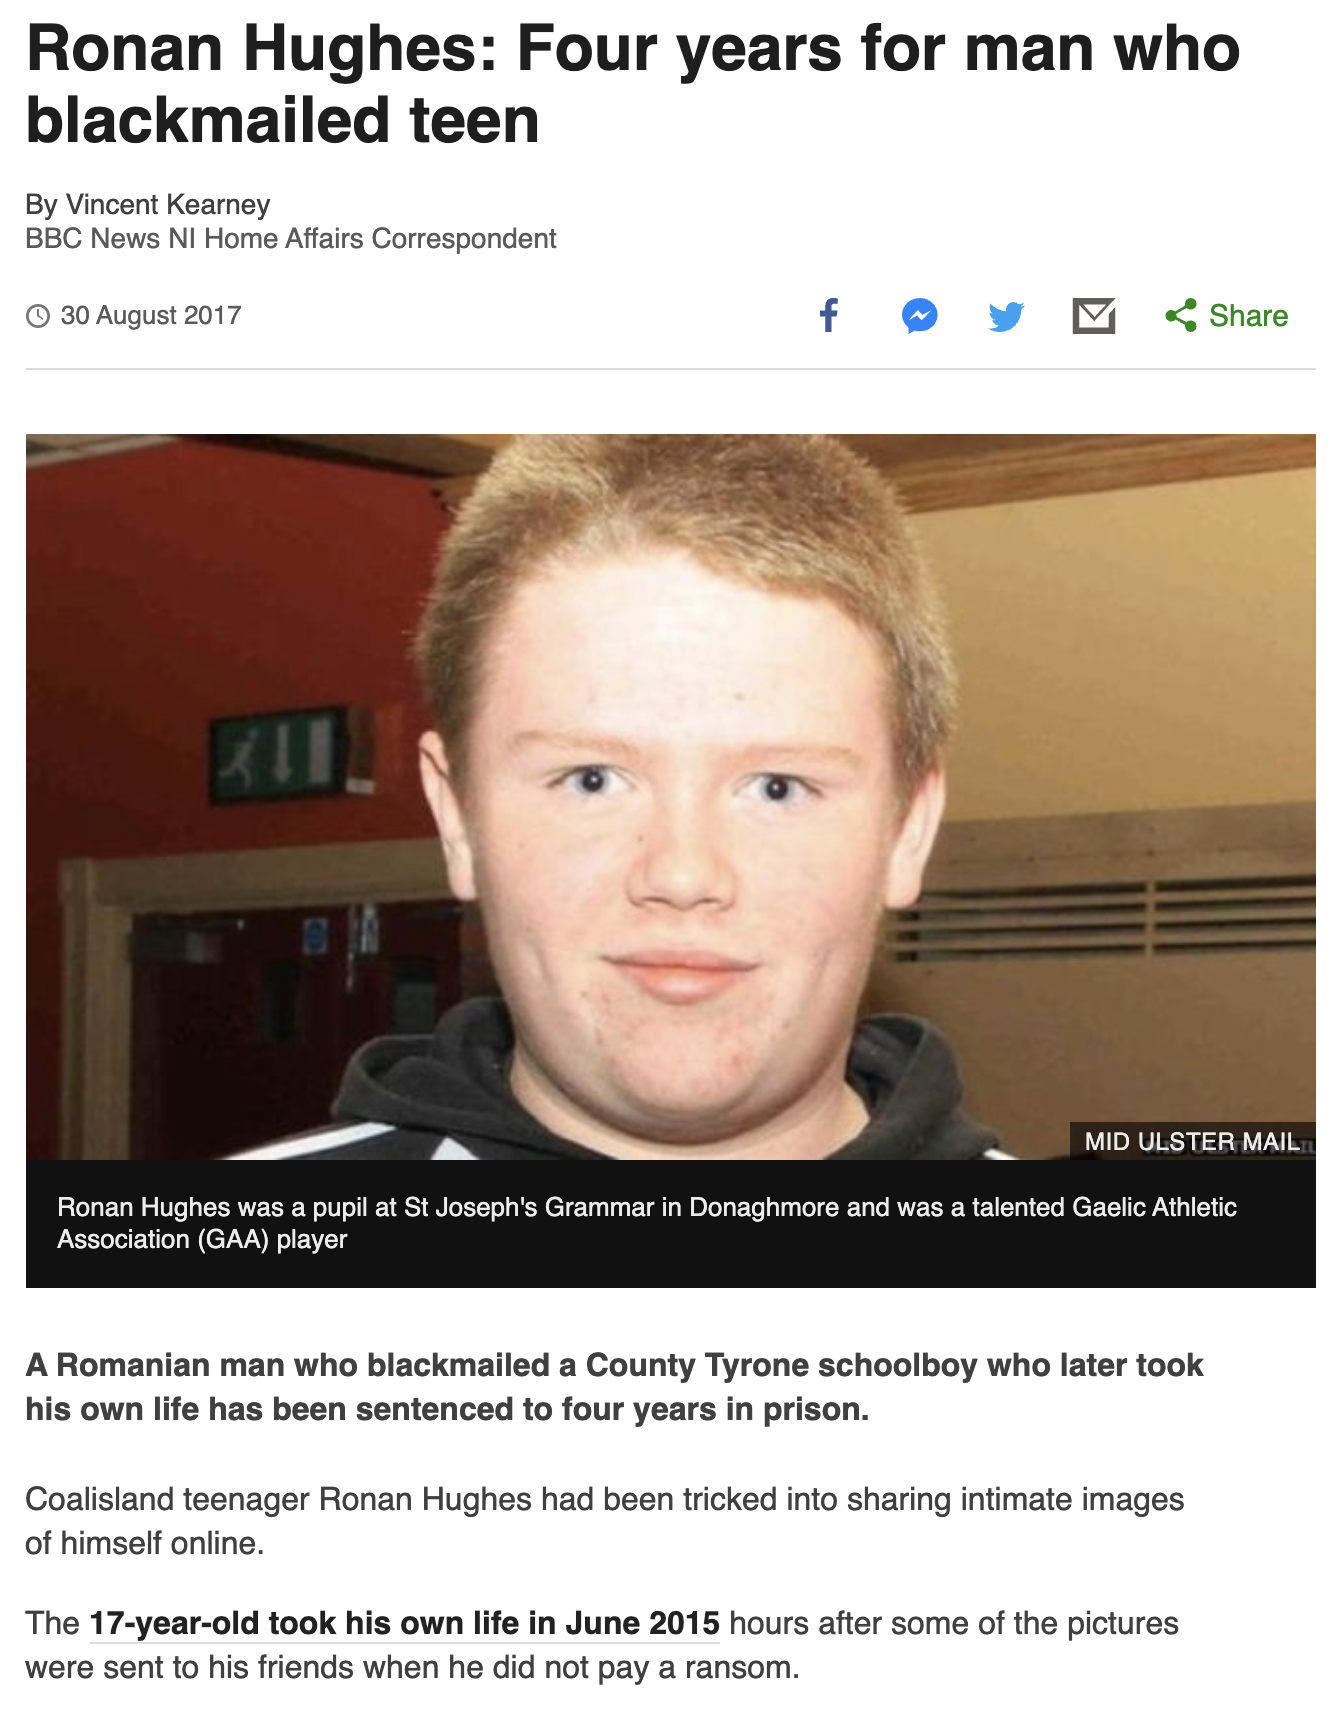
\includegraphics[width=\textwidth]{ronan-hughes-article}
            \end{figure}
        \column{0.5\textwidth}
            \begin{figure}
                \centering
                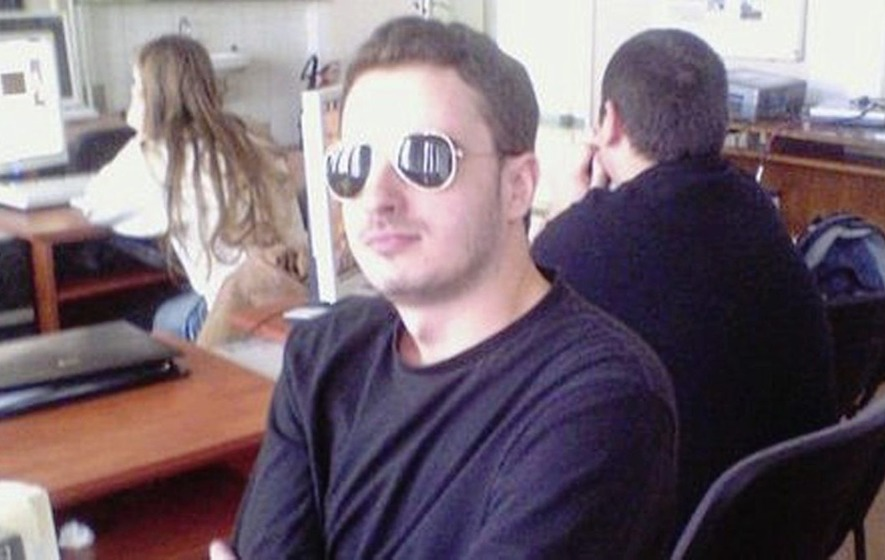
\includegraphics[width=\textwidth]{ronan-hughes-photo}
            \end{figure}
    \end{columns}
\end{frame}

\begin{frame}{Carter Clemons}
    \begin{figure}
        \centering
        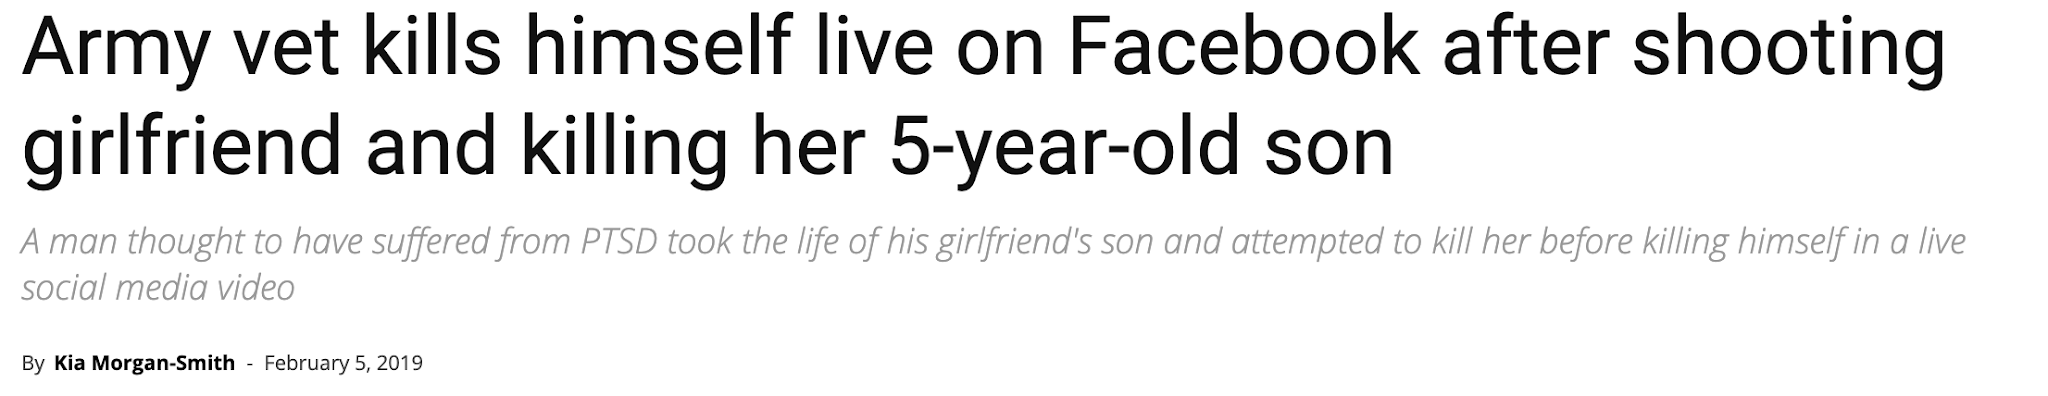
\includegraphics[width=\textwidth]{carter-clemons-news}
    \end{figure}
    \begin{columns}
        \column{0.5\textwidth}
            \begin{figure}
                \centering
                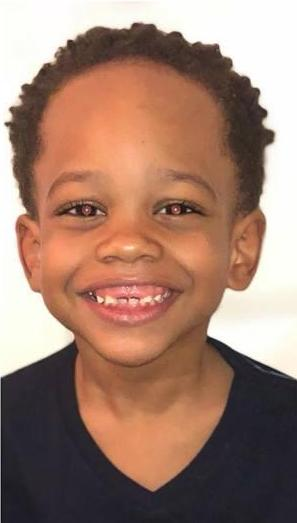
\includegraphics[height=0.6\textheight]{carter-clemons-son}
            \end{figure}
        \column{0.5\textwidth}
            \begin{figure}
                \centering
                
\includegraphics[height=0.5\textheight]{carter-clemons-photo}
            \end{figure}
    \end{columns}
\end{frame}

\begin{frame}{ISIS and Junaid Hussain}
    \begin{columns}
        \column{0.5\textwidth}
            \begin{figure}
                \centering
                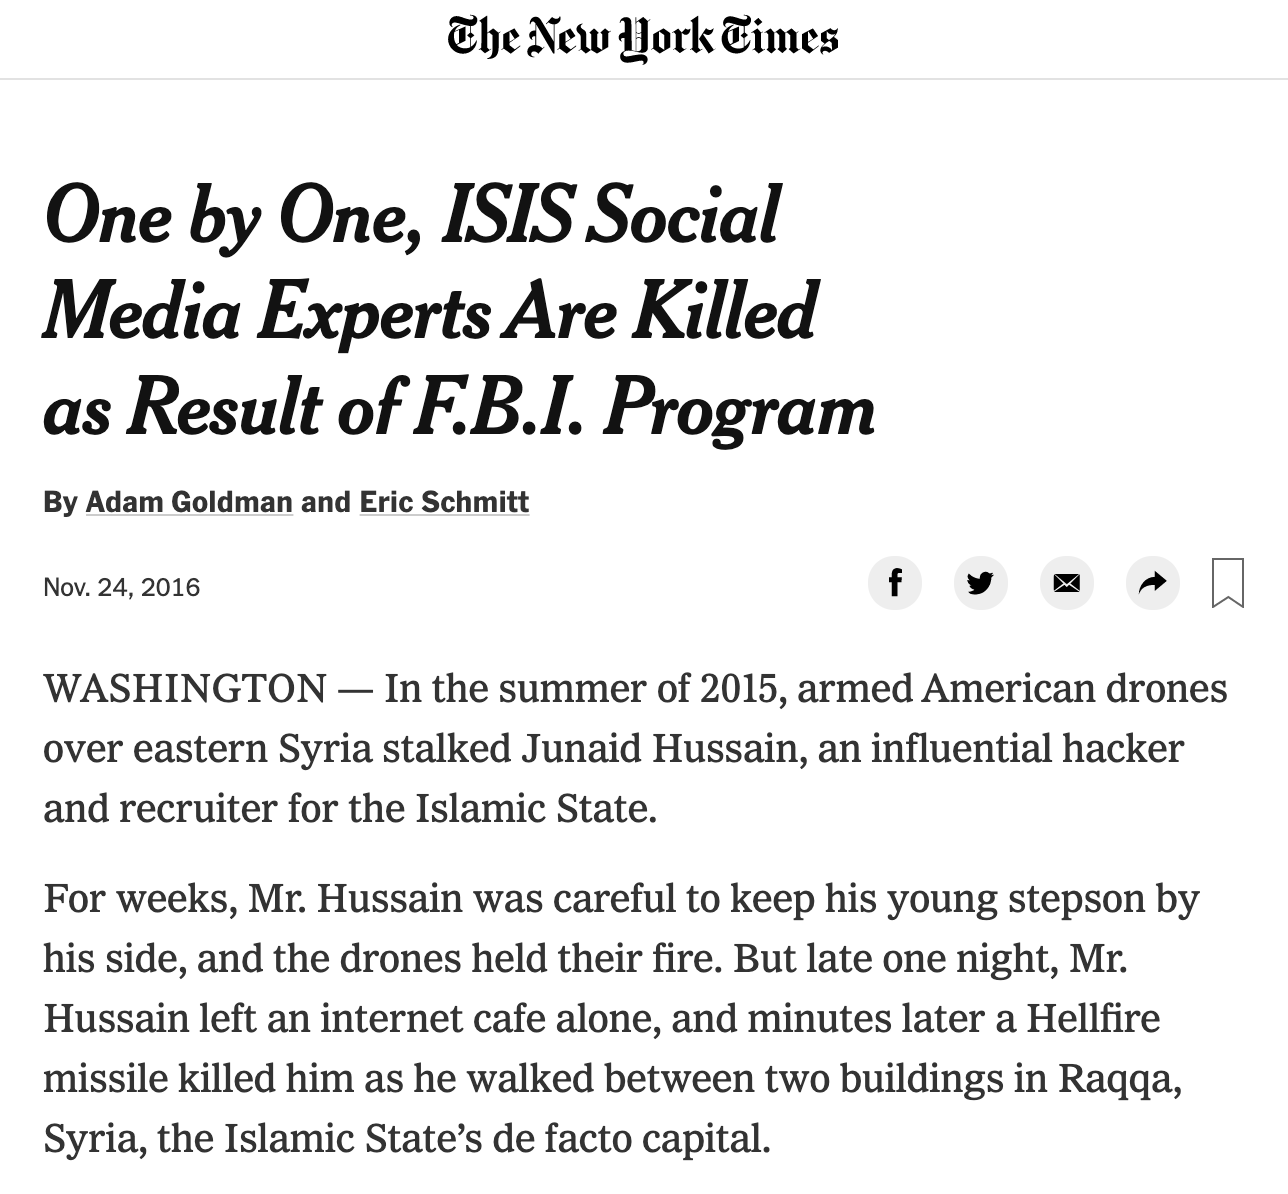
\includegraphics[width=\textwidth]{isis-nyt-article}
            \end{figure}
        \column{0.5\textwidth}
            \begin{figure}
                \centering
                
\includegraphics[width=\textwidth]{junaid-hussain}
            \end{figure}
            \vspace{0.5 cm}
            \begin{figure}
                \centering
                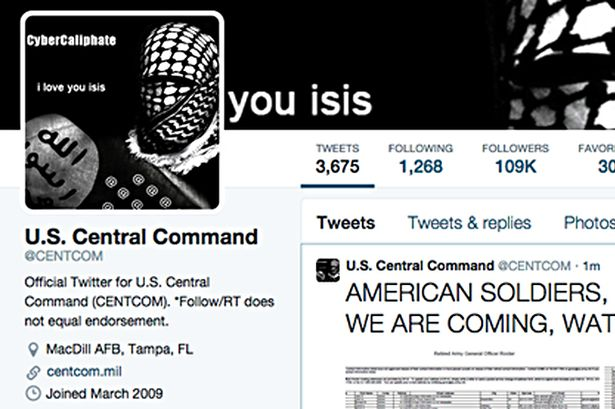
\includegraphics[width=\textwidth]{isis-twitter-hack}
            \end{figure}
    \end{columns}
\end{frame}

\begin{frame}{Buster Hernandez aka "Brian Kil"}
    \begin{columns}
        \column{0.6\textwidth}
            \begin{figure}
                \centering
                
\includegraphics[width=\textwidth]{brian-kil-headline}
            \end{figure}

            \begin{figure}
                \centering
                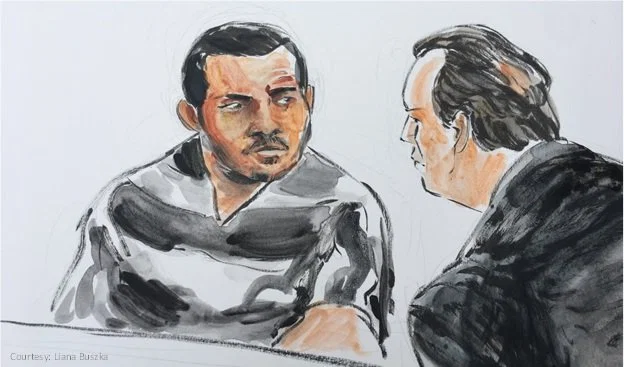
\includegraphics[width=\textwidth]{brian-kil-sketch}
            \end{figure}
        \column{0.4\textwidth}
            \begin{figure}
                \centering
                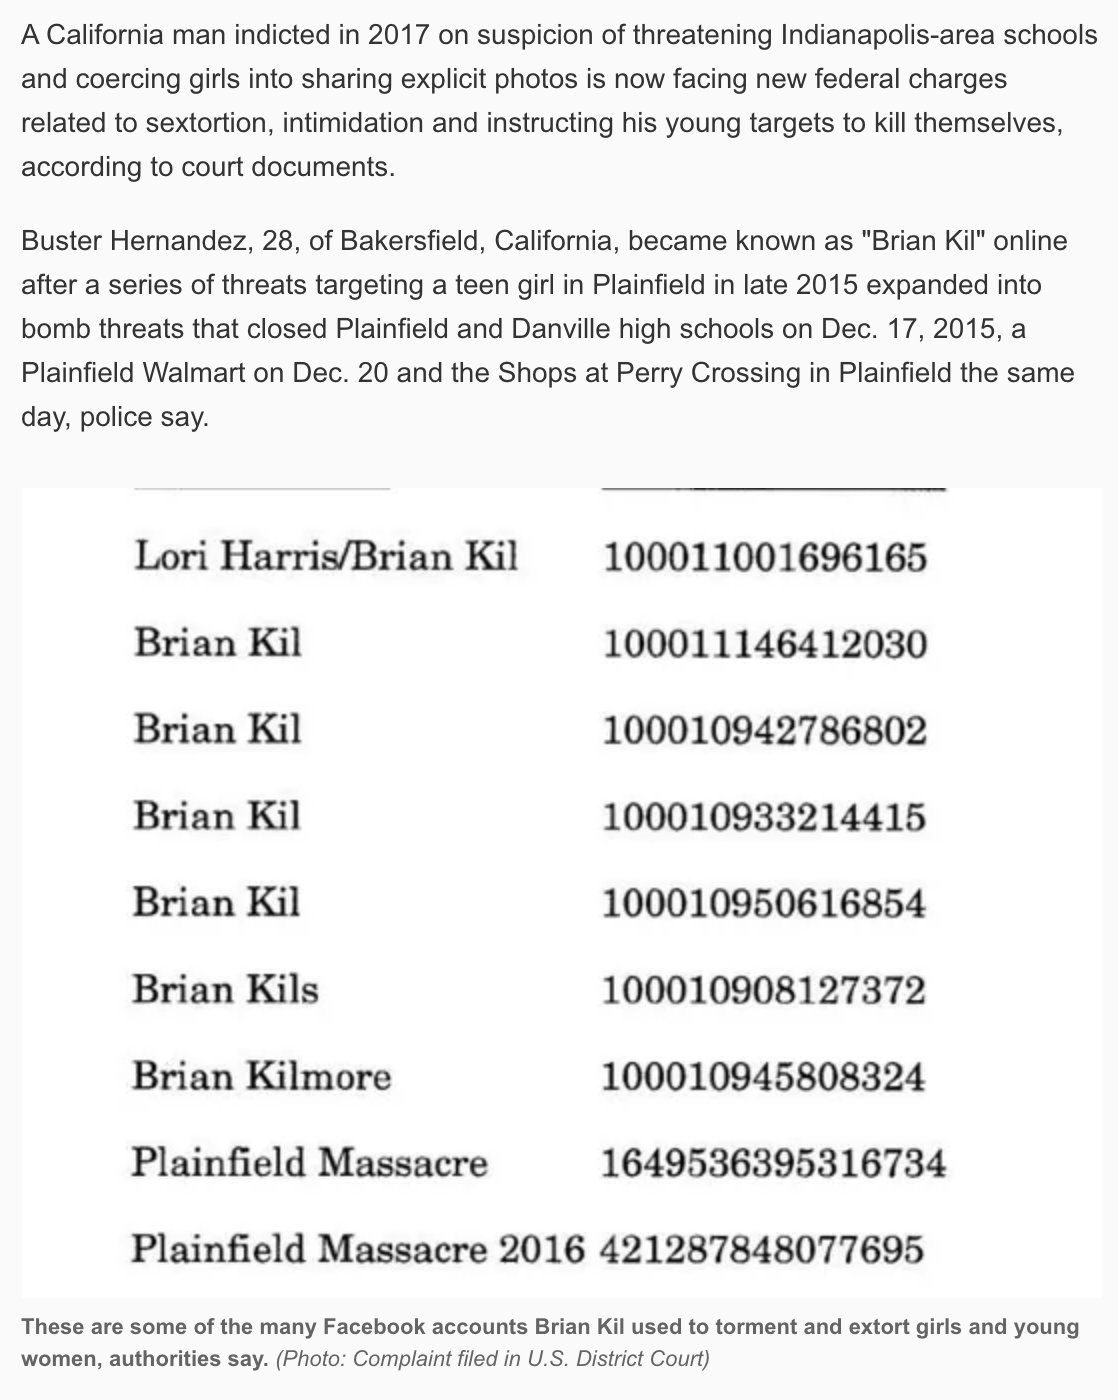
\includegraphics[width=\textwidth]{brian-kil-article}
            \end{figure}
    \end{columns}
\end{frame}

\begin{frame}{Zoe Quinn, Sarah Jeong and many others}
    \begin{columns}[T]
        \column{0.4\textwidth}
            \begin{figure}
                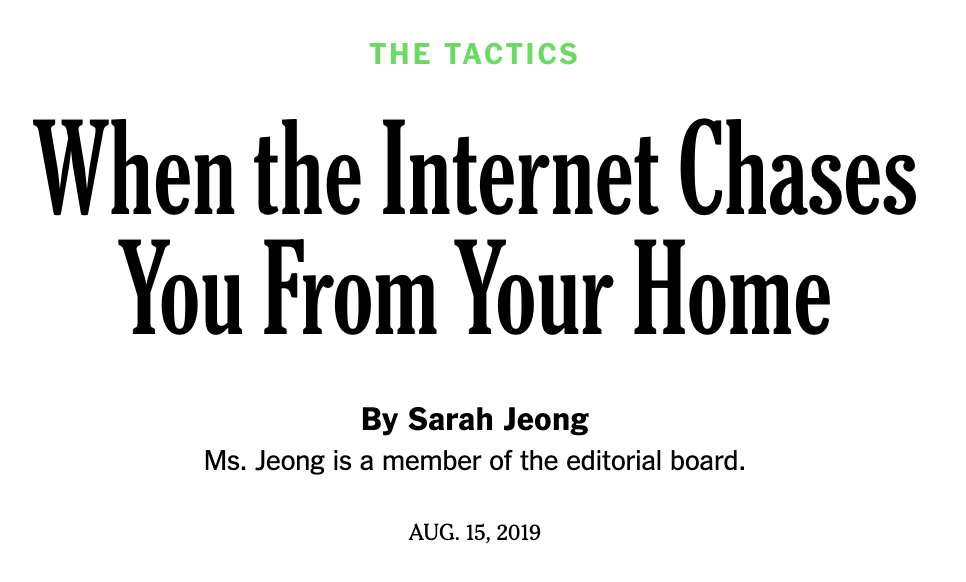
\includegraphics[width=\textwidth]{sarah-jeong-nyt-article}
            \end{figure}
        \column{0.6\textwidth}
            \begin{figure}
                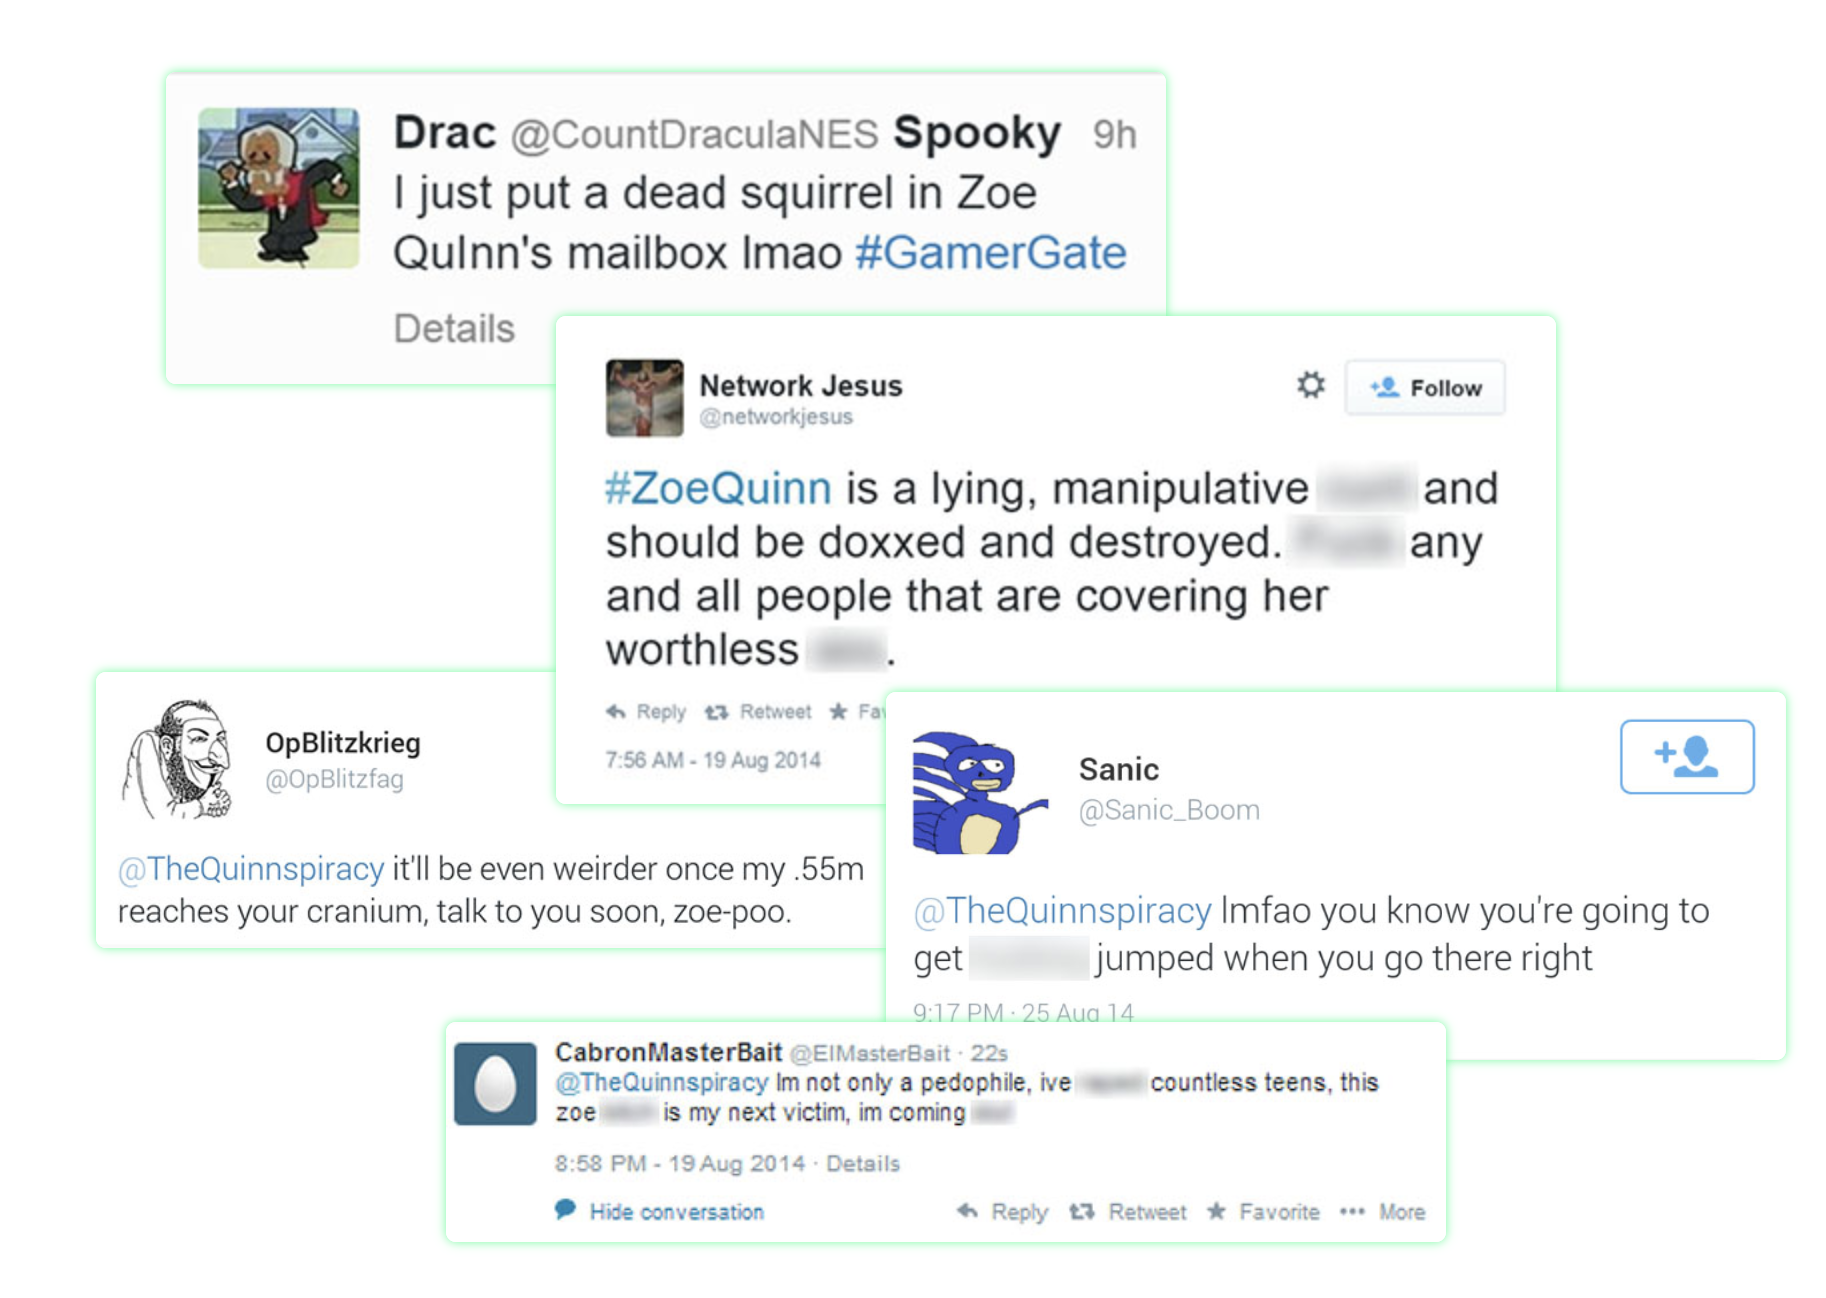
\includegraphics[width=\textwidth]{zoe-quinn-threatening-tweets}
            \end{figure}
    \end{columns}
    
    \tiny
    \url{https://www.nytimes.com/interactive/2019/08/15/opinion/gamergate-zoe-quinn.html}
\end{frame}

%TODO3: Questions slide
\section{Questions?}

\begin{frame}{}
    \thispagestyle{empty}
    Questions?
\end{frame}

\backpage

\end{document}

